\chapter{Introduction and Motivation}
\chapterquote{We can't focus on what's going wrong, there's always a way to turn things around.}{Joy, Inside Out}
Particle physics is the subject to study the fundamental structure of the universe. It is now based on the theory called the "Standard Model" (SM). It interprets the universe as the composition of tiny particles interacting with each other by the exchange of force carriers (another type of particle).  In July 2012, the discovery of Higgs boson made by the ATLAS and CMS collaboration \cite{HIGG-2012-27,CMS-HIG-12-028} completed SM 50 years after being predicted. By now, it has been deemed as one of the most successful theories in modern physics.
\\
\\
However, there are still some conflicts between the SM and factual results. For example, in the SM, neutrinos are supposed to be massless, but the discovery of neutrino oscillation support the fact that neutrinos are massive, and the SM cannot explain it. New theories are proposed in order to resolve those conflicts, and they indicate the existence of some new particles or the deviation from SM predictions. This thesis is dedicated to the work in search for this kind of new physics.
\section{Standard Model\cite{Griffiths,Perkins}}
The SM is a quantum field theory(QFT). In the QFT, the universe is filled with different fields, and all fundamental particles (particles without further substructure) are the forms of quantized fields. They make up the matters and also mediate interactions between them, which is the foundation how this universe operates. Those fundamental particles could be classified into two types: fermions and bosons. Fermions are the matter builders, while bosons are the force carriers exchanged between particles (for both fermions and bosons). 
\\
\\{\bf Fermions}
\\
\\Fermions are quantized from fermionic fields following Dirac-Fermi statistics with half integer spin number, $\pm\frac{1}{2}$. Under the statistic characteristic, fermions exclude each other with the same quantum status, which makes them different from bosons. \\
\\
All fermions have their counter antiparticles which in the SM have opposite charge and chirality. Those fermions are called "Driac Fermions". They can be presented as Weyl spinors of four components composed of one left-handed spinor and one right handed spinor following the Dirac equation. However, neutrinos, a sub-specie of fermions, have no counter-partner with opposite chirality found\footnote{Due to being neutral, although neutrinos and anti-neutronos were discovered, but neutrinos (anti-neutrinos) only have the left-handed (right-handed) chirality.}, so they are assumed to be "Majorana Fermions": they are their own antiparticle. They could be instead presented as Majorana spinors in Majorana equation. 
\\
\\{\bf Dirac Equation}: $i\hbar\gamma^{\mu}\partial_{\mu}\psi-mc\psi=0$ 
\\
\\{\bf Majorana Equation}: $i\hbar\gamma^\mu\partial_\mu\psi-mc\psi_c=0$
\\
\\$\psi$ is the fermion field with charge conjugate $\psi_c$, and $\gamma^\mu$ is the gamma matrix and m is the particle mass.
\\ 
\\Fermions can then be further categorized into two types, quarks and leptons, by the interactions they participate in. Quarks are the only particles involved in the strong interaction, so they cannot exist alone, and, instead, they are always in bound state as mesons of two quarks or baryons of three quarks. 
\\
\\Quarks have three generations (flavours) and six flavours. In each generation are quarks with different charges: $\frac{-1}{3}$ and $\frac{2}{3}$. The first generation are the lightest: up and down. Strange and charm are in the second generation. The third generation has bottom and top with highest mass. Quarks can change their flavour through CKM matrix relating to the weak interaction. The decay relation between quarks is shown in Fig.\ref{Fig:quarks}
\\    
\begin{figure}[!h]                
	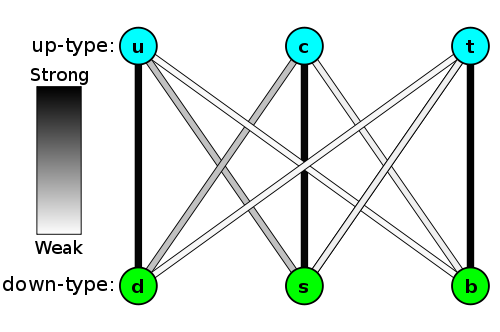
\includegraphics[width=0.45\textwidth]{Chapter1/quarks.png}
	\centering
	\begin{center}
		\caption{Relation between quarks are determined by CKM matrix taken from \cite{ckm_timothy}}
		\label{Fig:quarks}            
	\end{center}
\end{figure}

Similar to quarks, leptons also have 3 generations and 6 flavours. In each generation, there is one neutral neutrino and corresponding charged particle with charge -1. The three generations are electrons, muons and taus with their neutrino partners (among them, electron neutrino is assumed to be the lightest fundamental particle under normal hierarchy). Leptons participate in weak interaction, quantum electrodynamics(except for neutral neutrinos) and gravity. They can change flavours through PMNS matrix relating to the weak interaction.
\\
\\{\bf Interaction and Bosons}
\\
\\Under the SM, the interactions between particles are induced by gauge fields which could be quantized into gauge bosons. Different from fermions, those bosons follow Bose-Einstein statistics with integer spin number, which means more than one is allowed to occupy a single quantum state. They mediate interactions between particles including themselves. 
\\
\\Although there are four fundamental forces in the universe, only three of them are in SM, because they are quantizable: electromagnetic, weak and strong interactions. The challenge of quantizing gravity is still not achieved in modern physics. Each interaction has a part in the SM Lagrange formulism.
\\
\\The electromagnetic interaction is the best known among the four interactions. It is explained by quantum electrodynamics in the SM. The interaction is induced by electromagnetic field between two charged particles with charge as the invariance under $U(1)$ symmetry, which could be seen as they interchange photons. Because the electromagnetic interaction only occurs between charged particles, photon doesn't interact with neutral particles at the leading order \footnote{With a loop diagram, it can still be achieved by exchanging charged fermions between photons.}. The coupling constant (interaction strength which determines the possibility of a process  occurs) in the interaction is:
\\
\begin{equation}
\alpha_{EM} = \frac{e^2}{4\pi\hbar c}=\frac{1}{137.036...}
\end{equation}
\\
with $e$ as electric charge of electron, $\hbar$ as reduced Plank constant and $c$, the speed of light. Its part in the SM Lagrange could be written as:
\begin{equation}
\mathcal{L}=\bar{\psi}(i\gamma^{\mu}D_{\mu})\psi-F^{\mu\nu}F_{\mu\nu}
   \label{Eq:EM Lagrange}  
\end{equation}
In this equation, $\gamma^\mu$ is the Gamma matrices, $\psi$ is the Weyl spinor of spin $-\frac{1}{2}$ particles and $\bar{\psi}$ is the Dirac adjoint of $\psi$. $D_\mu=\partial_\mu+ieA_\mu+ieB_\mu$ represents the gauge covariant derivative with $e$ as the electric charge, $A_\mu$ as the filed induced by the particle itself and $B_\mu$ as the field from external source. In the equation, $F_{\mu\nu}$ is the electromagnetic field tensor. 
\\
\\All the left-handed particles participate in the weak interaction. It is mediated by three different bosons: the $W^+$, $W^-$ and $Z^0$ bosons. They are massive gauge bosons which obtain their mass via the electroweak symmetry breaking. The W boson is the mediator when a particle changes its flavour along with its charge, while Z boson is involved in the neutral current interactions which leave the particles unchanged with only kinematic momentum transfer. Within this process, a quantity, isospin, is conserved under $SU_L(2)$ symmetry. Its definition is similar to the spin numbers of a pair of electrons in the same orbital. For two fermions in the same generations, their quantum states are identical except for isospin which is opposite of them to each other. As right-handed fermions don't participate in weak interaction, their isospin is 0. The isospins of fermions are showed in Table.\ref{Tab:isospin}. 
\\


\begin{table}[h]
	\caption{Isospin of Elementary fermions}
	\renewcommand{\arraystretch}{1.2}
	\centering
	\begin{tabular}{l c c c c r}
		\hline
		\hline
		1st Generation &Isospin        &2nd Generation    &Isospin        &3rd Generation   &Isospin\\
		\hline
		$e^-$          &$-\frac{1}{2}$ &$\mu^-$           &$-\frac{1}{2}$ &$\tau$           &$-\frac{1}{2}$\\
		\hline
		$\nu_e$        &$\frac{1}{2}$  &$\nu_\mu$         &$\frac{1}{2}$  &$\nu_\tau$       &$\frac{1}{2}$\\
		\hline
		$u$            &$\frac{1}{2}$  &$c$               &$\frac{1}{2}$  &$t$              &$\frac{1}{2}$\\
		\hline
		$d$            &$-\frac{1}{2}$ &$s$               &$-\frac{1}{2}$ &$b$              &$-\frac{1}{2}$\\
		\hline

	\end{tabular}
    \label{Tab:isospin}
\end{table}
\noindent
The coupling constant for weak interaction is defined as:
\begin{equation}
\alpha_{W} = \frac{g_{W}}{4\pi\hbar c}\approx\frac{1}{29}
\end{equation}
with $g_{W}$ as the W weak charge strength. In terms of the interactions via Z boson, it is substituted by Z weak charge, $g_{Z}$. A unification between the weak and electromagnetic interactions could be achieved with another new parameter called electroweak hypercharge defined as $Y_w=2 (Q-I_3)$ where $I_3$ is isospin and $Q$ is the electric charge under $SU_L(2)\times U(1)$ symmetry in the scale of high energy.  In SM, the symmetry would be spontaneously broken by the Higgs field to give particles mass. It will be discussed in the next section.
\\
\\Only quarks are involved in the strong interaction which is described by quantum chromodynamics(QCD). The conserved quantity in the interaction is also imaginary, colour, with gluons as the force carrier boson under $SU(3)$ symmetry. There are three different colours: red, blue and green along with their anti-colour partners. Similar to the principle of light, the colour would be absent when the three colours are mixed together or with their anti-colour, and it is the condition for a stable state in QCD. Each quark is only allowed to carry one colour, but this state is unstable. It needs to be bound with another quarks to stabilize the system, and they exchange gluons to form the bounding force. In QCD, gluons have 8 types with different colour combinations:
\begin{equation}
         (r\bar{b}+b\bar{r})/\sqrt{2}, \quad -i(r\bar{b}-b\bar{r})/\sqrt{2}  \\
         (r\bar{g}+g\bar{r})/\sqrt{2}, \quad -i(r\bar{g}-g\bar{r}/\sqrt{2})  \\
          (b\bar{g}+g\bar{b})/\sqrt{2},\quad -i(b\bar{g}-g\bar{b}/\sqrt{2})   \\
          (r\bar{r}-b\bar{b})/\sqrt{2},\quad  (r\bar{r}+b\bar{b}-2g\bar{g})/\sqrt{6}
\end{equation}
with $r$, red charge, $b$, blue charge, and $g$, green charge.
\\
\\Different from the other interactions, the colour confinement of gluon self-interaction makes the effective potential increase linearly with the distance between two colour-charged particles. Under this process, the potential energy decays into a quark-antiquark pair, and it is repeated also within the newly produced pair. This leads to the divergence of with the perturbative strong coupling constant, and the mathematical technique, ``renormalization'', is introduced to solve the problem. 
\\
\\Its part of the SM Lagrange could be shown as:
\begin{equation}
\mathcal{L}_{QCD}=\bar{\psi}(i(\gamma^\mu D_\mu)_{ij}-m\delta_{ij})\psi_j-\frac{1}{4}G^a_{\mu\nu}G_a^{\mu\nu} 
\end{equation}
with
\begin{equation}
G^a_{\mu\nu}=\partial_\mu\mathcal{A}^a_\mu-\partial_\nu\mathcal{A}^a_\nu+gf^{abc}\mathcal{A}^b_\mu\mathcal{A}^c_\nu 
\end{equation}
with $\psi_i$, the quark field in $SU(3)$ representation indexed of i,j, ..., $G^a_{\mu\nu}$, the gluon field also in $SU(3)$ representation indexed of a, b... from 1 to 8. $f^{abc}$ is the structure constant, $\mathcal{A}_\mu$ is the spin 1 gluon filed and $g = \sqrt{4\pi\alpha_s}$ is the QCD coupling constant.
\\
\\All the elementary particles with their basic properties are shown in Fig. \ref{Fig:elementary_particle}. The 3 interactions with their conserved quantities makes SM under the gauge theory with the gauge group with $U(1) \times SU(2)_L \times SU(3)$ gauge group.

\begin{figure}[!h]                
	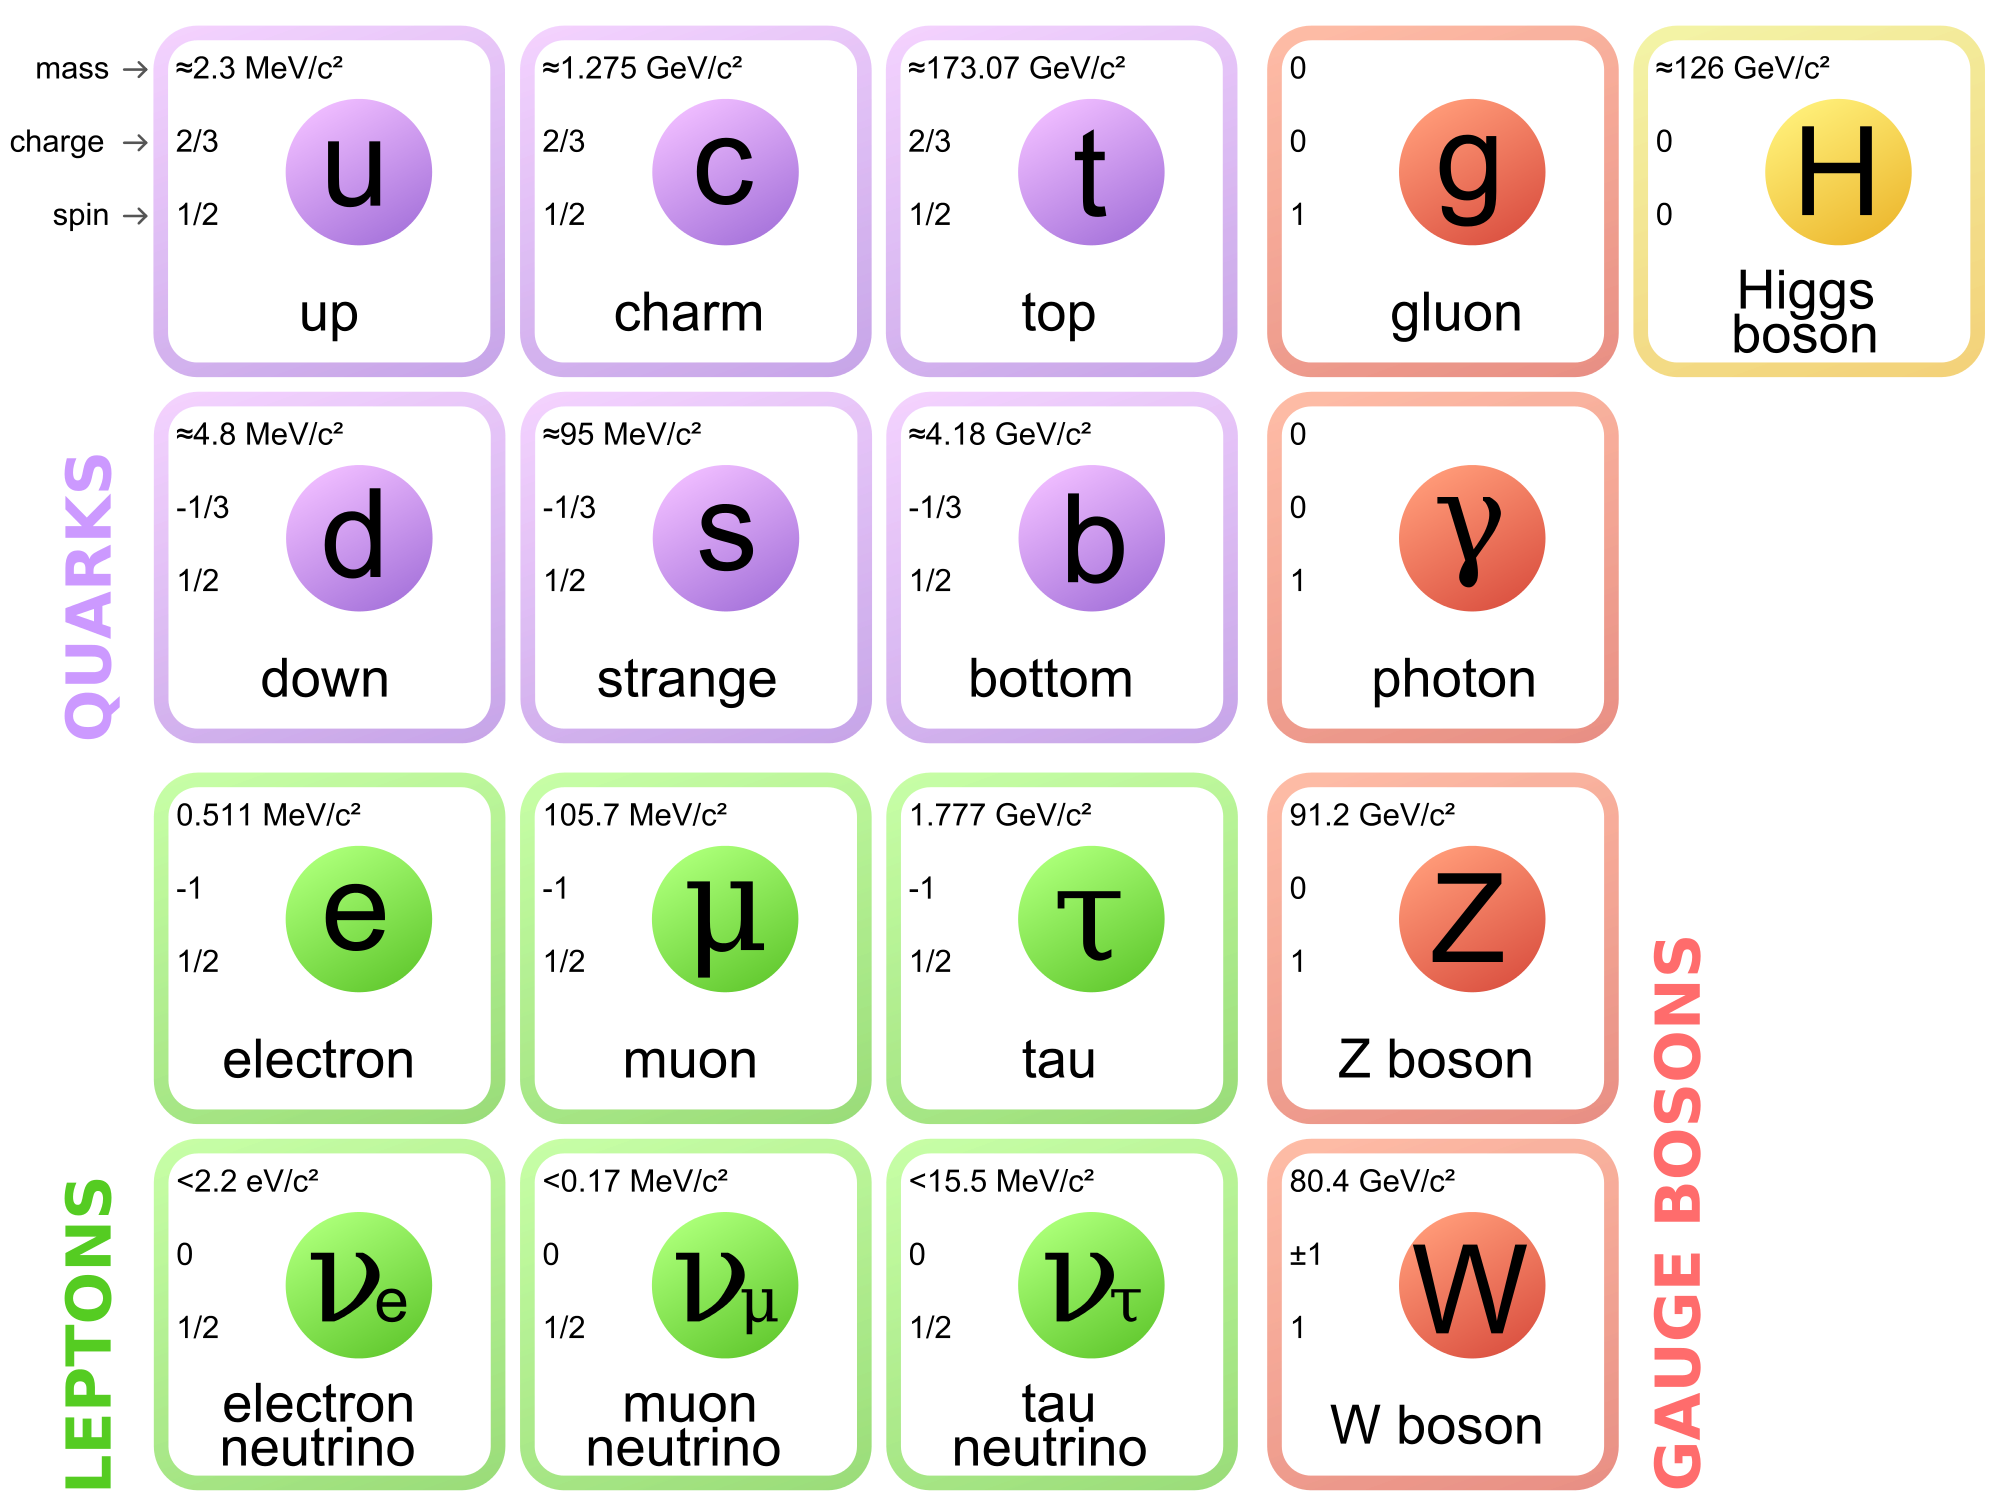
\includegraphics[width=0.9\textwidth]{Chapter1/elementary_particle.png}
	\centering
	\begin{center}
		\caption{Elementary particles and properties taken from \cite{SMParticle}}
		\label{Fig:elementary_particle}            
	\end{center}
\end{figure}

\section{Electroweak Symmetry Breaking}
One particle in Fig. \ref{Fig:elementary_particle} is not mentioned yet: Higgs boson, the last discovered fundamental particle in the SM. It arises from quantized Higgs field which was proposed by three groups in early 1960s:  Robert Brout and Francois Englert\cite{Englert}, Peter Higgs\cite{Higgs} as well as Gerald Guralnik, C. R. Hagen, and Tom Kibble\cite{Hagen}. It induces spontaneous electroweak symmetry breaking via the ''Brout-Englert-Higgs mechanism``.  The Higgs boson discovery was announced on 4th July 2012 and confirmed on 14 March 2013 with spin 0 and $+$ parity by the ATLAS and CMS collaboration.
\\
\\The Higgs field is defined as the scalar gauge field in a complex scalar $SU(2)_L$ doublet :
\begin{equation}
 \Phi= \left(  \begin{array}{ c } \phi^+\\  \phi^0 \end{array} \right) 
\end{equation}
The potential for field is:
\begin{equation}
 V(\Phi)=\mu^2|\Phi^\dagger\Phi|+\lambda(|\Phi^\dagger\Phi|)^2
\label{Eq:sm_higgs_potential}
\end{equation}
For some value of $\mu$ and $\lambda$, the minimal potential can be at $\Phi = 0$, and the shape of the potential would be as Fig. \ref{Fig:V} (this is a simplified plot, and the real one should be in 4 dimensions). In this potential, the symmetry is not broken with the minimal value at $\Phi = 0$.
\\ 
\begin{figure}[!h]                
	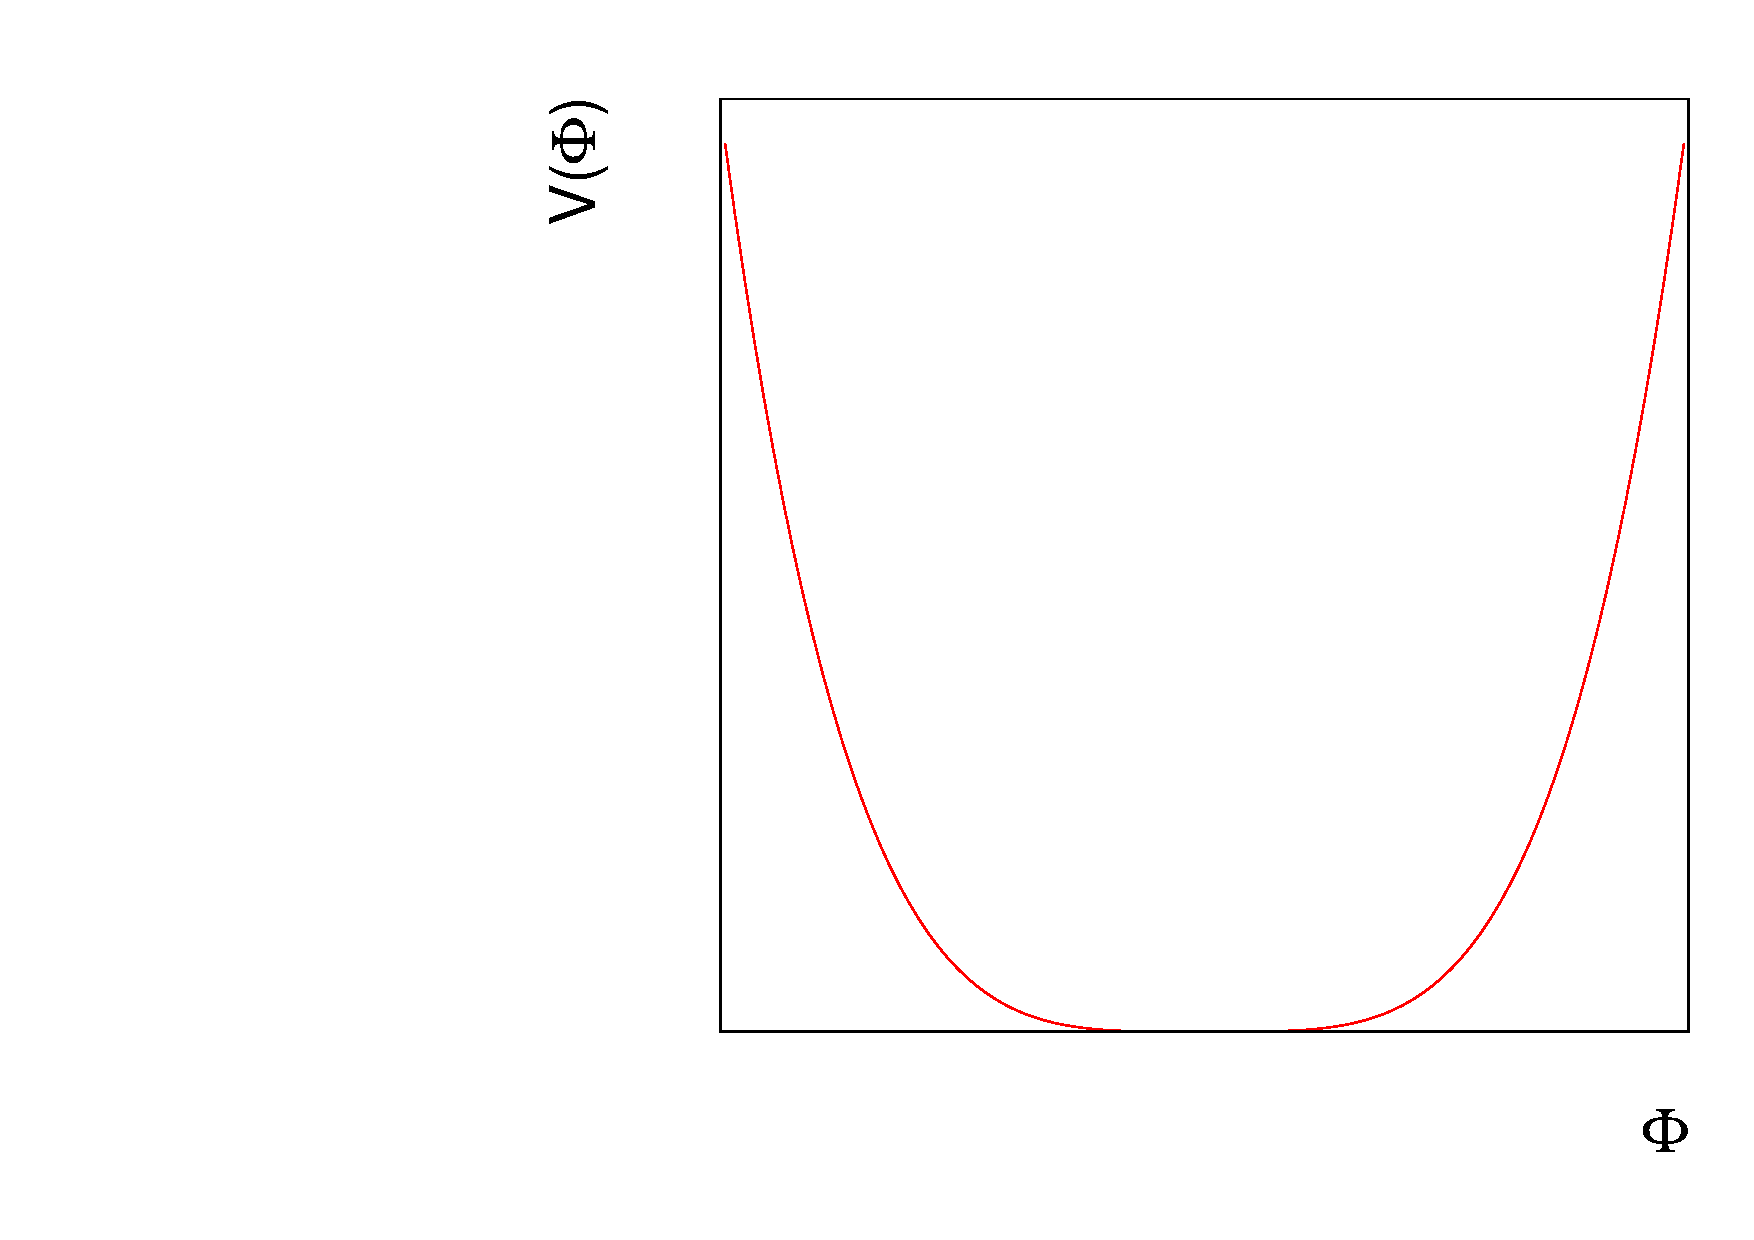
\includegraphics[width=0.4\textwidth]{Chapter1/V.pdf}
	\centering
	\begin{center}
		\caption{Scalar potential with $\mu^2 > 0$}
		\label{Fig:V}            
	\end{center}
\end{figure}
\\In an alternative scenario for $\mu^2 < 0$, the potential shape becomes Fig. \ref{Fig:higgs}. The minimal expected value of the potential is not at 0 but at:
\begin{equation}
\label{Eq:min}
\langle\Phi\rangle=\sqrt{-\frac{\mu^2}{2\lambda}}\left ( \begin{array}{c} 0 \\ 1 \end{array} \right) \equiv\frac{\nu}{\sqrt{2}}\left ( \begin{array}{c} 0 \\ 1 \end{array} \right)
\end{equation}
The potential is only affected by $|\Phi^\star\Phi|$, so the shape of the potential is determined by the real term (imaginary terms are cancelled out). The value in Eq.~\ref{Eq:min} is called the "vacuum expectation value"(VEV). To maintain a stable state, particles are only allowed to stay in the lowest potential, the valley part. This makes the degree of freedom of the particles decrease from four to one and breaks the $SU_L(2)\times U(1)$ symmetry with isospin and hypercharge to $U(1)$ symmetry with electric charge.  
\begin{figure}[!h]                
	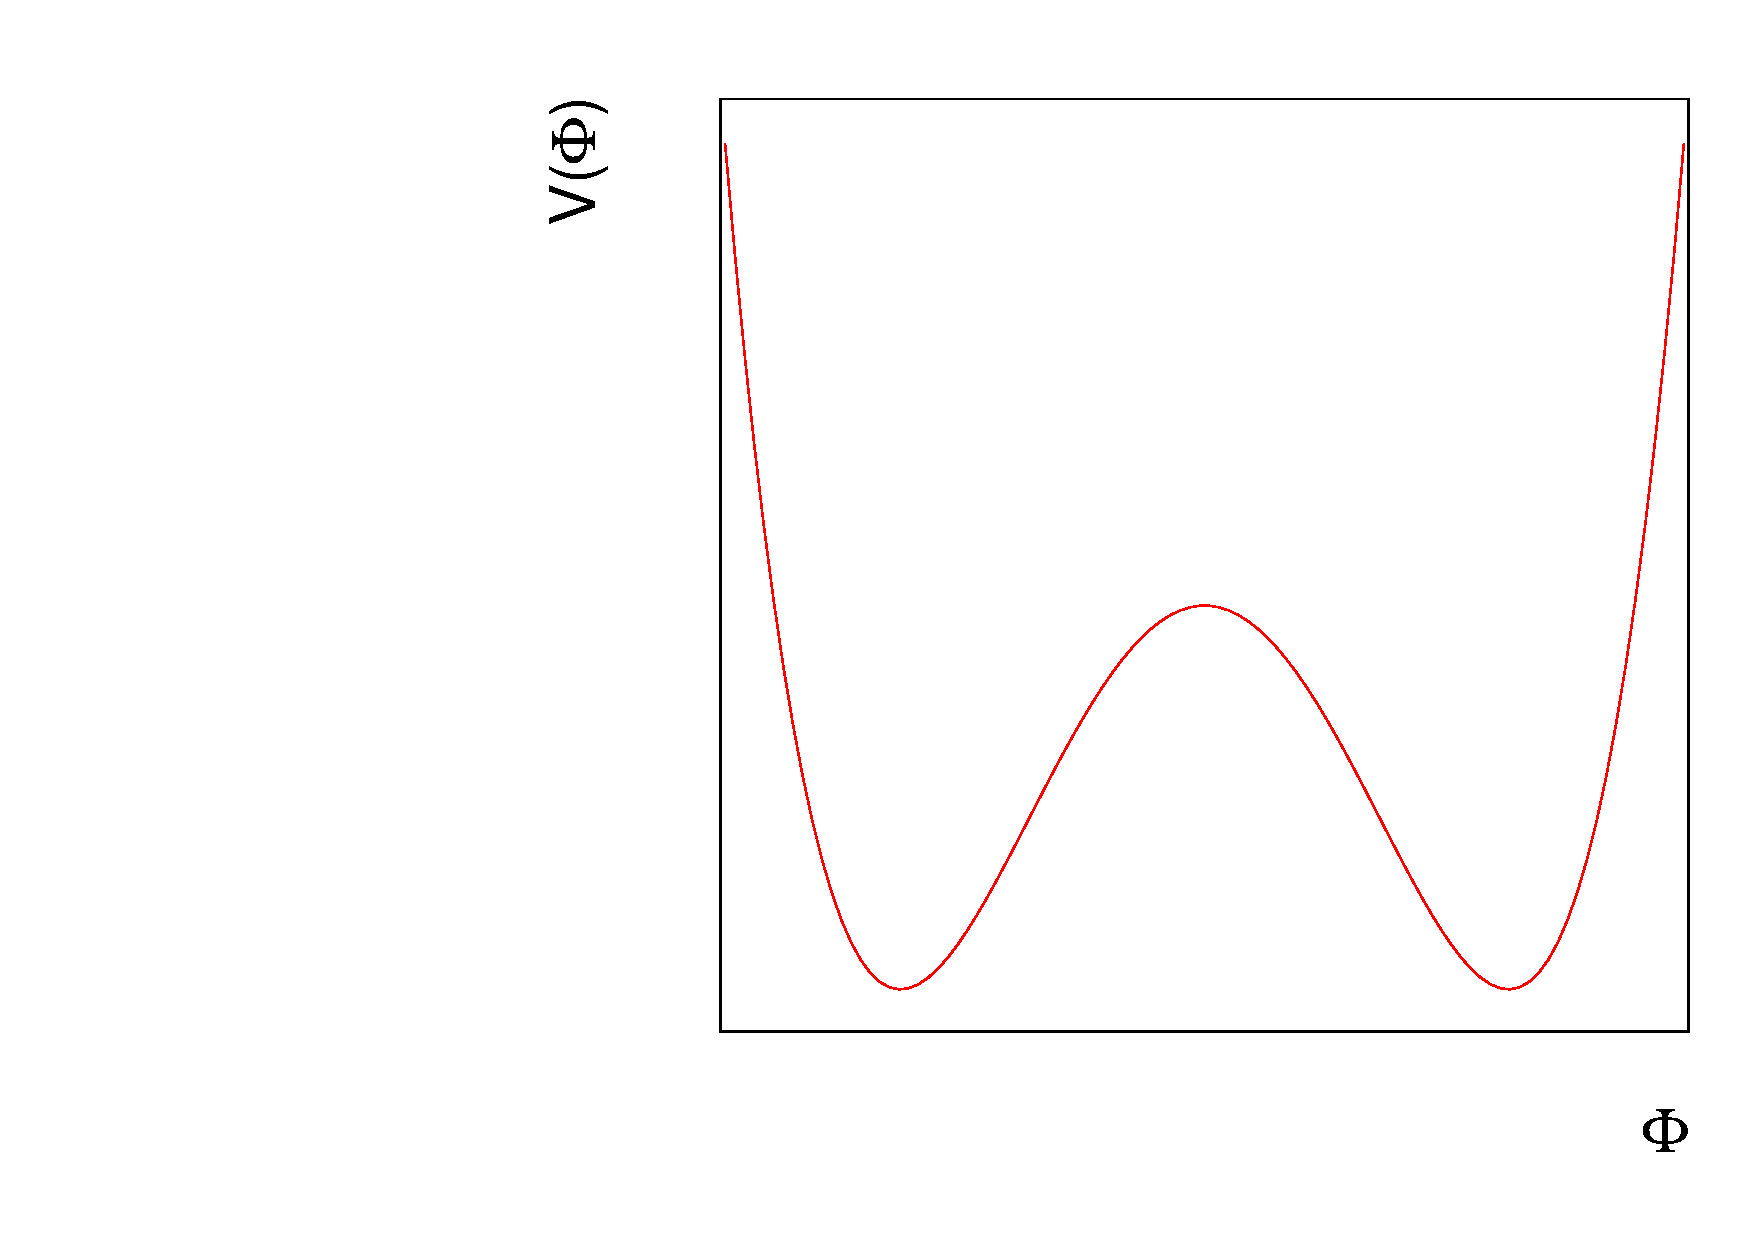
\includegraphics[width=0.4\textwidth]{Chapter1/higgs.pdf}
	\centering
	\begin{center}
		\caption{Scalar potential with $\mu^2 < 0$}
		\label{Fig:higgs}            
	\end{center}
\end{figure}
In high energy regime above the valley (excited state), electromagnetic and weak interaction are mixed together to form three $SU_L(2)$ gauge bosons, $W^i_\mu$ with $\mu =1,2,3$ and one $U(1)$ gauge boson, $B_\mu$. They are not SM particles, but they could be taken as the excited form of SM gauge bosons. The Lagrangian for the interaction between them and Higgs field is:
\begin{equation}
 \mathcal{L}=(D^\mu\Phi)^\dagger(D_\mu\Phi) - V(\Phi) 
\end{equation}
with
\begin{equation}
 D_\mu = \partial_\mu+i\frac{g}{2}\tau\cdot W_\mu+i\frac{g'}{2}B_\mu Y
 \label{Eq:electroweak symmetry Lagrange}  
\end{equation}
$g$ and $g'$ are the coupling constants between the fields, $\tau$ is the Pauli matrix and Y is the hypercharge.
\\
\\A unitary gauge transformation on the Higgs field can remove Goldstone bosons\footnote{Unitary gauge transformation is to select the fixed gauge which sets the Goldstone boson terms into 0} after the symmetry breaking. The Higgs field is thus shifted with the new gauge as:
\begin{equation}
\Phi=\frac{\nu+h}{\sqrt{2}}\left ( \begin{array}{c} 0 \\ 1 \end{array} \right)
\end{equation}
with h, the physical Higgs sector, as a complex number.
\\
\\After inserting the new Higgs field into and rearranging SM Lagrange, the SM gauge bosons could be shown as:  
\begin{equation}
W^{\pm}_\mu=\frac{1}{\sqrt{2}}(W^{1}_\mu\mp iW^{2}_\mu) 
\end{equation}
\begin{equation}
Z^\mu=\frac{-g'B_\mu+gW^3_\mu}{\sqrt{g^2+g'^2}} 
\end{equation}
\begin{equation}
A^\mu=\frac{gB_\mu+g'W^3_\mu}{\sqrt{g'^2+g^2}} 
\end{equation}
with particle masses:
\begin{equation}
M^2_W=\frac{1}{4}g^2\nu^2 
\end{equation}
\begin{equation}
M^2_Z =\frac{1}{4}(g^2+g'^2)\nu^2 
\end{equation}
\begin{equation}
M_A=0 
\end{equation}
From the expression, it turns out that $Z$ boson and photon are both the mix of $B$ and $W^3$ bosons with different phases which could be shown as:
\begin{equation}
 \left[ \begin{array}{c}  A \\ Z \end{array} \right]=\left[ \begin{array}{l r} cos\theta_W &  sin\theta_W \\ -sin\theta_W & cos\theta_W \end{array} \right]\left[ \begin{array}{c}  B\\ W^3 \end{array} \right] 
  \label{Eq:AZ phase}  
\end{equation}
With $\cos{\theta_W}=\frac{g}{\sqrt{g^2+g'^2}}$ and $\sin{\theta_W}=\frac{g'}{\sqrt{g^2+g'^2}}$. Here, $\theta_W$ is called the weak mixing angle or Weinberg angle. By this, the electroweak parameter, $\rho$, is defined:
\begin{equation}
\label{Eq:rho}
\rho = \frac{m_W}{m_Z\cos{\theta_W}} 
\end{equation}
\\with the comparison between Eq. \ref{Eq:EM Lagrange} and Eq. \ref{Eq:electroweak symmetry Lagrange} with Eq. \ref{Eq:AZ phase}, the electric charge could be defined as:
\begin{equation}
e=g\sin{\theta_W}=g'\cos{\theta_W}
\end{equation}
\\This relation gives the access to a precision measurement of $\rho$, which is now given ~1.0008, a litte deviation from expectation of 1 in the SM because of the loop diagram correction.
\\
\\In terms of degrees of freedom, before symmetry breaking, its comes with four degrees from Higgs complex scalar doublet, six degrees from $SU(2)_L$ gauge field, $W_i$, and two degrees from $U(1)_Y$ gauge field, $B$, which makes 12 degrees in total for all the massless fields. After symmetry breaking, the number of degrees of freedom doesn't reduce with nine degrees from three massive vector boson, $Z$ and $W_{\pm}$, two degrees from massless photon,A, and one degree from physical real scalar field, $h$.
\\
\\Not only granting mass to bosons, the interaction between fermions and Higgs boson is also part of the Brout-Englert-Higgs Mechanism. The left-handed fermionic field is defined as a doublet:
\begin{equation}
 Q_L=\left(  \begin{array}{ c } u_L\\  d_L \end{array} \right)
\end{equation}
For right-handed leptons, the representation would be in a singlet because of the lack of right-handed neutrinos.      
\\
\\Their interaction with Higgs field are through Yukawa couplings\footnote{Yukawa coupling means the couplings betweent fermionic and bosonic fields}
\begin{equation}
\mathcal{L} = -\lambda\bar{Q_L}\Phi d_R + h.c. 
\end{equation}
with $\lambda$ as the coupling constant. The Lagrangian can lead to the quark mass as:
\begin{equation}
 m_d=\frac{\lambda \nu}{\sqrt{2}}
\end{equation}
This mechanism would change the chirality of a fermion, when it is giving the mass. However, no right-handed neutrino and left-handed anti-neutrino were measured, which leaves it as one of the unsolved problem in SM. (More details are given in next section.)
\section{Unsolved Problems in SM}
With SM, we have understood most behaviours of the fundamental particles. However, it still failed explaining some experimental results. The following is part of the them the work in the thesis is trying to answer.
\\
\\{\bf Higgs Mass Naturalness\cite{WILLIAMS201582}}
\\
\\In quantum field theory, all the experimental observables could be presented as:
\begin{equation}
O=a_1+a_2+a_3+...
\end{equation}
where O corresponds to the physical observables like the invariant mass of particles, and $a_n's$ are the independent contributions to the observables. For naturalness of the observable, it is expected that $a_n\leq O$. For any case that $a_n>>0$, the further fine-tuning needs to be introduced for proper correction on theory, and it also indicates the defect in the theory. \\
\\The form for the observable of Higgs mass is:
\begin{equation}
m_h^2=2\mu^2+\delta m_h^2
\end{equation}
where $\delta m_h^2$ for the contribution from coupling to top quark is:
\begin{equation}
\delta m_h^2 \simeq \frac{3}{4\pi^2}\left(\lambda^2_t+\frac{g^2}{4}+\frac{g^2}{8\cos^2{\theta_w}}+\lambda\right)\Lambda
\end{equation}
where $\lambda_t$ is the top-quark Yukawa coupling, g is the $SU\left(2\right)$ gauge coupling, $\lambda$ is the the coupling constant in the quadratic term in Higgs potential and $\lambda$ is the energy cut-off to divergent loop integrals. With the observed Higgs boson mass at 125$GeV$, $\Lambda$ is estimated to be around 1$TeV$, and that is also roughly the limit to keep the naturalness of this observable. 
\\
\\However, many models beyond the SM predicts the existence of particles at the TeV scale, which means the naturalness would be broken in the scenario. For this reason, a correction for Brout-Englert-Higgs Mechanism is needed, or there is possibly a heavier Higgs boson to complete the theory.  
\\
\\{\bf The Hierarchy Problem and Quantum Gravity\cite{BenA}}
\\
\\The hierarchy problem is defined in two ways: the unreasonable discrepancy between theoretical prediction and experimental result, or two comparable parameters. Higgs mass is one instance for the first definition. For the second one, it is generally referred to the gap between coupling strengths of weak interaction and gravity for the order of $10^{16}$.
\\
\\When a hierarchy problems occurs, the ``so-called'' fine-tuning is introduced to correct the discrepancy between two parameters. However, the fine-tinning could only be performed with enough understanding on the quantum effect of related parameters, and quantum gravity is still an unsolved problem. In the case, no solution is available.
\\
\\{\bf Neutrino Mass}
\\
\\Brout-Englert-Higgs Mechanism is the process to make particles massive within which the chirality of fermions would be changed. This implies that massive fermions of right-handed and left-handed chirality shall both exist, but no evidence is found for right handed neutrinos (or left-handed anti-neutrinos). Therefore, they are supposed be massless with SM. However, with the measurement of neutrino oscillation\cite{SuperK} induced by the difference of neutrino mass and flavour eigenstates, they are practically massive particles. The conflict between SM and experiment still remains unsolved.
\section{Thesis Overview}
To solve the problems in SM, analyses are performed in two ways, resonance and non-resonance searches which are corresponding to two different signatures in physics: new particles or new couplings. The thesis will present how the experiment is set up to see the signatures of new physics in Chapter \ref{chap:exp}, and the following three chapters are dedicated to show the analyses of resonance and non-resonance searches with 2015+2016 data corresponding to the integrated luminosity of $36.1~fb^{-1}$for which I made the contributions to the multijet background estimation, study on trigger performance, data background comparison, analysis framework development, and the statistical interpretation. The last chapter is for the simulation of the upgrade of the LHC and ATLAS detector which will start to operate in 2021. I made the contribution to the construction of the simulation framework along with the supporting components and also the study for the preliminary missing transverse energy ($E^{miss}_{T}$, the definition will be shown later) trigger.

